% !TeX program = pdflatex
% Un Motor, Tres Recuentos -- Descartes, Sturm, Budan-Fourier a traves de un solo motor
% de variacion de signos en Lean 4. Version en espanol de sign-variation-lean.tex.
% Sin babel (rompe tikz/math); acentos con \' y [utf8]{inputenc}. Build: pdflatex (dos veces).

\documentclass[11pt]{article}
\usepackage[T1]{fontenc}
\usepackage[utf8]{inputenc}
\usepackage{lmodern}
\usepackage{amsmath,amssymb,amsthm,booktabs,graphicx,hyperref}
\usepackage{xurl}
\usepackage[table]{xcolor}
\definecolor{ggteal}{HTML}{1B6F8C}
\definecolor{ggband}{HTML}{DCE7EB}
\definecolor{ggamber}{HTML}{E08A1E}
\definecolor{ggplum}{HTML}{7B4B94}
\usepackage[margin=1in]{geometry}
\usepackage{microtype}
\usepackage{float}
\usepackage[most]{tcolorbox}
\usepackage{tikz}
\usetikzlibrary{arrows.meta,positioning,fit,backgrounds,matrix}
\graphicspath{{figures/}}
\setlength{\emergencystretch}{3em}
\newtheorem{theorem}{Teorema}
\newtheorem{proposition}{Proposici\'on}
\newtheorem{remark}{Observaci\'on}
\newcommand{\lean}[1]{{\def\_{\textunderscore\allowbreak}\texttt{#1}}}
\newcommand{\R}{\mathbb{R}}
\newcommand{\V}{\mathrm{V}}
\hypersetup{colorlinks=true,linkcolor=ggteal,citecolor=ggteal,urlcolor=ggteal}
\newtcbox{\keybox}{on line,boxrule=0.9pt,colframe=ggteal,colback=ggband!40,
  arc=3pt,left=8pt,right=8pt,top=5pt,bottom=5pt}
\newcommand{\keyeq}[1]{\begin{center}\keybox{$\displaystyle #1$}\end{center}}
\newtcolorbox{recipebox}[1]{colframe=ggamber,colback=ggamber!8,arc=3pt,boxrule=0.8pt,
  title=\textbf{#1},coltitle=white,colbacktitle=ggamber}

\title{\bf Un Motor, Tres Recuentos\\[4pt]
  \large\normalfont Descartes, Sturm y Budan--Fourier a trav\'es de un solo motor de variaci\'on de
  signos en Lean~4}
\author{Carles Mar\'in\thanks{Formalizado con la asistencia de un sistema de IA (Claude, Anthropic);
la matem\'atica es cl\'asica, toda afirmaci\'on, delimitaci\'on de alcance y limitaci\'on es
responsabilidad del autor, y es el n\'ucleo de Lean---no el asistente---quien certifica las pruebas. La
frontera entre lo cl\'asico y lo aportado aqu\'i se traza expl\'icitamente en la
Secci\'on~\ref{sec:ours}.}\\[3pt]
  \normalsize Investigador independiente\\
  \normalsize \texttt{karlesmarin@gmail.com}}
\date{Junio de 2026}

\begin{document}
\maketitle

\begin{abstract}
Tres teoremas cl\'asicos cuentan las ra\'ices reales de un polinomio en un intervalo leyendo las
variaciones de signo de una secuencia: la regla de \emph{Descartes} usa los coeficientes,
\emph{Budan--Fourier} la torre de derivadas $p,p',p'',\dots$, y \emph{Sturm} la cadena de restos
firmados. Que sean facetas de un mismo principio es cl\'asico (Akritas~\cite{akritas};
Basu--Pollack--Roy~\cite{bpr}), y el invariante unificador m\'as profundo, el \'indice de Cauchy, se
axiomatiza mediante las \emph{cadenas de Sturm} abstractas de Eisermann~\cite{eisermann} y est\'a
verificado por m\'aquina, para la v\'ia del \'indice de Cauchy, en Isabelle/HOL por Li y
Paulson~\cite{liCauchy}. Este paper hace tres cosas en Lean~4 sobre Mathlib, todas \lean{sorry}-free.
(1)~Exhibe \emph{un solo motor}---un recuento de variaciones de signo, su constancia local fuera de los
puntos cr\'iticos, y un telescopaje global sobre ellos---y hace pasar los tres teoremas por \'el: las
primeras formalizaciones en Lean del teorema de Sturm~\cite{sturmlean} y del teorema de
Budan--Fourier~\cite{budanlean}, y el puente \lean{fourierVar p 0 = Polynomial.signVariations p} que
identifica el $\V(0)$ del motor con el recuento de signos de coeficientes de la propia regla de
Descartes de Mathlib, de modo que el tercer recuento tambi\'en se verifica contra la biblioteca y no
se lee solo en prosa. (2)~Enuncia su ley de ca\'ida local com\'un, $\V(c^-)=\V(c^+)+\mu_c+2e$, donde
$\mu_c$ es el orden con que el polinomio contado se anula en el punto cr\'itico $c$. (3)~Localiza con
precisi\'on d\'onde divergen los tres: el axioma de cadena de Sturm de Eisermann proh\'ibe que dos
miembros consecutivos se anulen a la vez, y la torre de derivadas lo \emph{viola} en cada ra\'iz
m\'ultiple, de modo que la torre \emph{no} es una cadena de Sturm---su ley local es el
colapso/alternancia por bloques (\lean{Rseq}/\lean{Lseq}), de la que la ca\'ida antipodal de una
cadena de Sturm genuina es el caso especial no degenerado. La unificaci\'on es cl\'asica; la
contribuci\'on es el motor compartido en Lean, las dos primeras formalizaciones en Lean que carga, el
puente de Descartes con el recuento de coeficientes de Mathlib, y esta colocaci\'on axiom\'atica exacta
de la torre. Todo teorema cabecera depende solo de \lean{propext}, \lean{Classical.choice},
\lean{Quot.sound}.
\end{abstract}

\medskip
\noindent Tres teoremas, nacidos con siglo y medio de diferencia, cuentan ra\'ices reales con el mismo
gesto: leer los signos de una secuencia. Descartes (1637) los ley\'o en los \emph{coeficientes} y acot\'o
las ra\'ices positivas. Budan (1807) y Fourier (a\~nos 1820, publicado p\'ostumamente en 1831) los
leyeron en la \emph{torre de derivadas}, extendiendo la cota a cualquier intervalo y contando con
multiplicidad; su descubrimiento casi simult\'aneo desat\'o una disputa de prioridad que m\'as tarde
desenred\'o Akritas~\cite{akritas}. Sturm (1829) cerr\'o la brecha de cota a recuento \emph{exacto}---pero
con una tercera secuencia, los restos eucl\'ideos firmados, y solo para ra\'ices distintas. Que estas
sean tres caras de un mismo principio no emergi\'o hasta el siglo XX, a trav\'es del \'indice de Cauchy
y su axiomatizaci\'on moderna como \emph{cadenas de Sturm} abstractas por Eisermann~\cite{eisermann}.
\textbf{Este paper hace concreta esa fusi\'on en Lean: un motor de variaci\'on de signos, una ley de
ca\'ida local, tres instancias que pasan por \'el, y el punto exacto donde la torre de derivadas sale
del mundo de las cadenas de Sturm.} La unificaci\'on es cl\'asica; lo nuevo es el motor verificado por
m\'aquina y la l\'inea axiom\'atica que permite trazar entre los tres.

\medskip
\noindent\emph{Lo que encontrar\'as aqu\'i.} Un motor (Secci\'on~\ref{sec:engine}); la ley de ca\'ida
local que comparten (Secci\'on~\ref{sec:law}); las tres instancias le\'idas en \'el---Descartes, Sturm,
Budan--Fourier (Secci\'on~\ref{sec:three}); la l\'inea divisoria, donde la torre abandona el mundo de
las cadenas de Sturm (Secci\'on~\ref{sec:divide}); qu\'e es cl\'asico y qu\'e se aporta, sin adornos
(Secci\'on~\ref{sec:ours}); y las preguntas que merece la pena llevarse (Secci\'on~\ref{sec:open}). Los
dos papers compa\~neros~\cite{sturmlean,budanlean} cargan las pruebas completas de las instancias de
Sturm y Budan--Fourier; aqu\'i los ensamblo en una sola imagen y trazo la l\'inea entre ellos.

\begin{figure}[htbp]
\centering
\resizebox{\textwidth}{!}{%
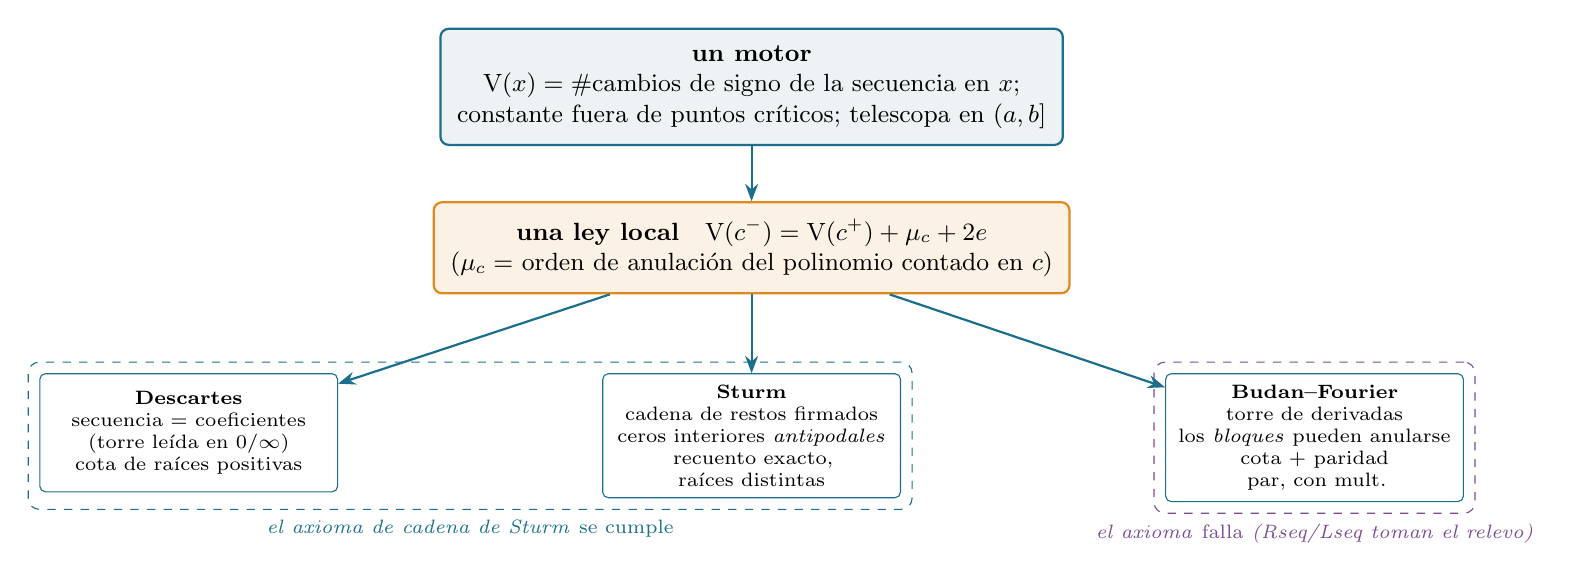
\begin{tikzpicture}[
  eng/.style={draw=ggteal,thick,rounded corners=3pt,fill=ggband!50,align=center,font=\small,
    inner sep=6pt},
  inst/.style={draw=ggteal,rounded corners=2pt,align=center,font=\scriptsize,inner sep=4pt,
    minimum height=15mm,text width=35mm,fill=white},
  law/.style={draw=ggamber,thick,rounded corners=3pt,fill=ggamber!12,align=center,font=\small,
    inner sep=6pt},
  arr/.style={-{Stealth[length=2.2mm]},thick,ggteal}]
  \node[eng] (engine) {\textbf{un motor}\\$\V(x)=\#$cambios de signo de la secuencia en $x$;\\
    constante fuera de puntos cr\'iticos; telescopa en $(a,b]$};
  \node[law,below=7mm of engine] (law)
    {\textbf{una ley local}\quad $\V(c^-)=\V(c^+)+\mu_c+2e$\\
     ($\mu_c=$ orden de anulaci\'on del polinomio contado en $c$)};
  \node[inst,below left=10mm and 12mm of law] (desc)
    {\textbf{Descartes}\\secuencia $=$ coeficientes\\(torre le\'ida en $0$/$\infty$)\\cota de ra\'ices positivas};
  \node[inst,below=10mm of law] (sturm)
    {\textbf{Sturm}\\cadena de restos firmados\\ceros interiores \emph{antipodales}\\recuento exacto, ra\'ices distintas};
  \node[inst,below right=10mm and 12mm of law] (bf)
    {\textbf{Budan--Fourier}\\torre de derivadas\\los \emph{bloques} pueden anularse\\cota $+$ paridad par, con mult.};
  \draw[arr] (engine) -- (law);
  \draw[arr] (law) -- (desc);
  \draw[arr] (law) -- (sturm);
  \draw[arr] (law) -- (bf);
  \begin{scope}[on background layer]
    \node[fit=(desc)(sturm),draw=ggteal,dashed,rounded corners=4pt,inner sep=4pt,
      label={[font=\scriptsize\itshape,text=ggteal]below:el axioma de cadena de Sturm \emph{se cumple}}] {};
    \node[fit=(bf),draw=ggplum,dashed,rounded corners=4pt,inner sep=4pt,
      label={[font=\scriptsize\itshape,text=ggplum]below:el axioma \emph{falla} (Rseq/Lseq toman el relevo)}] {};
  \end{scope}
\end{tikzpicture}}
\caption{La tesis en una imagen. Un solo motor de variaci\'on de signos y una sola ley de ca\'ida local
cargan tres recuentos cl\'asicos de ra\'ices. Las secuencias de Descartes y Sturm obedecen el axioma de
cadena de Sturm de Eisermann---no hay dos miembros que se anulen juntos; la torre de derivadas de
Budan--Fourier lo rompe en cada ra\'iz m\'ultiple y necesita la ley por bloques \lean{Rseq}/\lean{Lseq},
de la que el caso antipodal es una degeneraci\'on.}
\label{fig:thesis}
\end{figure}

\section{Un motor}\label{sec:engine}

Fija una secuencia finita de polinomios reales $S=(S_0,\dots,S_n)$ y, para un punto $x$ que no sea una
obstrucci\'on com\'un, sea
\[
  \V_S(x)\ =\ \#\{\text{cambios de signo en } (\mathrm{sign}\,S_0(x),\dots,\mathrm{sign}\,S_n(x)),\ \text{ceros eliminados}\}.
\]
En Lean esto es una sola funci\'on, \lean{signChanges} sobre la lista de signos evaluados (equivalentemente
\lean{signVarAt} sobre los polinomios), con un \'unico motor de paridad \lean{wallCount} por debajo. Dos
hechos valen para \emph{cualquier} secuencia de funciones continuas y se prueban una vez: \emph{(i)} en un
intervalo donde ning\'un miembro se anula, todo signo es constante, as\'i que $\V_S$ es localmente constante
(\lean{signVarAt\_eq\_of\_no\_root}, por el teorema del valor intermedio); \emph{(ii)} la paridad de $\V_S$
en un bloque con extremos sin ceros depende solo de su primer y \'ultimo signo supervivientes
(\lean{wallCount\_even\_iff\_endpoints}). Los \emph{puntos cr\'iticos}---donde alg\'un miembro se anula---son
finitos (las ra\'ices de $\prod_k S_k$, un polinomio no nulo), as\'i que $\V_S$ es una escalera: plana entre
cr\'iticos, y el descenso total sobre $(a,b]$ telescopa en una suma de ca\'idas por cr\'itico. Esta espina
se comparte verbatim entre los tres teoremas; se escribi\'o una vez y se us\'o tres.

\section{Una ley local}\label{sec:law}

Todo se reduce entonces a la ca\'ida a trav\'es de un \'unico punto cr\'itico $c$. Escribe
$\V(c^-),\V(c^+)$ para los valores localmente constantes justo a la izquierda y la derecha de $c$, y sea
$\mu_c$ el orden con que el polinomio \emph{contado} (la cabeza $S_0=p$) se anula en $c$. Los tres teoremas
son instancias de un enunciado.
\keyeq{\V(c^-)\ =\ \V(c^+)\ +\ \mu_c\ +\ 2e\qquad(\exists\,e\in\mathbb{N}).}
El lado derecho no lleva informaci\'on m\'as all\'a de $c$ (el recuento justo a la derecha iguala el
recuento en $c$ con los ceros ignorados); el lado izquierdo a\~nade el orden de anulaci\'on $\mu_c$ de la
cabeza y un excedente \emph{par} $2e$ del interior. Sumando sobre los puntos cr\'iticos en $(a,b]$ se obtiene
el enunciado de intervalo: el n\'umero de ra\'ices de $p$ all\'i (con multiplicidad $=\sum\mu_c$) es a lo sumo
$\V(a)-\V(b)$, y difiere de \'el por el par $\sum 2e$. Toda la divergencia entre los tres teoremas est\'a en
\emph{c\'omo se comporta el interior}---y eso es exactamente lo que separan las dos secciones siguientes.

\section{Tres instancias}\label{sec:three}

Las leemos las tres en un polinomio trabajado donde se pueden comparar, $p=x^3-x=x(x-1)(x+1)$, y luego
nombramos el rasgo que cada una a\'isla.

\emph{Sturm} (\cite{sturmlean}; Figura~\ref{fig:compare}). La cadena de restos firmados
$x^3{-}x,\ 3x^2{-}1,\ \tfrac23 x,\ 1$ se construye de modo que los miembros consecutivos sean coprimos: en
un cero de un miembro interior los dos vecinos son \emph{antipodales} (estrictamente opuestos), as\'i que
borrar ese miembro deja el recuento sin cambio (la relaci\'on \lean{FlankReduce}). Solo el par cabeza
$(p,p')$ mueve el recuento, en uno, en cada ra\'iz. La ca\'ida cuenta las ra\'ices \emph{distintas} de forma
exacta: $\V(-2)-\V(2)=3$ en $(-2,2]$. Aqu\'i $\mu_c=1$ en cada ra\'iz y el excedente es $0$.

\emph{Budan--Fourier} (\cite{budanlean}; Figura~\ref{fig:compare}). La torre de derivadas $p,p',p'',\dots$
reemplaza la coprimalidad por una relaci\'on de un paso---cada miembro es la derivada del anterior---as\'i
que el signo de un miembro que se anula justo fuera de $c$ queda fijado por su derivada: lo copia a la
derecha (el bloque \emph{colapsa}, sin cambio nuevo) y lo niega a la izquierda (el bloque \emph{alterna}, un
cambio por miembro). En una ra\'iz m\'ultiple se anula un bloque entero, la alternancia de la izquierda aporta
la multiplicidad, y los bloques interiores aportan un excedente par---as\'i que el recuento es una
\emph{cota con multiplicidad}, par-desviada de la verdad. Para $x^3-x$ (ra\'ices simples) coincide con Sturm;
su cara distintiva es la ra\'iz doble y la ca\'ida par fantasma (Figura~\ref{fig:compare}).

\emph{Descartes} es la sombra en los extremos de $(0,\infty)$: como $p^{(k)}(0)=k!\,a_k$, la secuencia de
signos de la torre en $0$ \emph{es} la secuencia de coeficientes, as\'i que $\V(0)$ es el recuento de
variaciones de signo de los coeficientes; y $\V(+\infty)=0$. La cota de ra\'ices positivas es
$\V(0)-\V(+\infty)=\V(0)$, par-desviada de la verdad. Para $x^3-x$ los coeficientes $1,0,-1,0$ dan un cambio
de signo y una ra\'iz positiva, $x=1$. Esta \'ultima instancia se verifica contra la biblioteca, no solo se
afirma: \lean{fourierVar p 0 = Polynomial.signVariations p} (\lean{Descartes.lean}, \lean{sorry}-free), de
modo que el $\V(0)$ del motor es \emph{por definici\'on} el propio recuento de variaciones de signo de
coeficientes de Mathlib---la funci\'on sobre la que est\'a enunciada la regla de Descartes de Mathlib. El
puente son los dos hechos de arriba ($p^{(k)}(0)=k!\,a_k$, y $\V(+\infty)=0$ dejado a la prosa) junto con la
invariancia por reversi\'on del recuento de signos, listando la torre los signos de menor a mayor y la lista
de coeficientes de Mathlib de mayor a menor.

\begin{figure}[htbp]
\centering
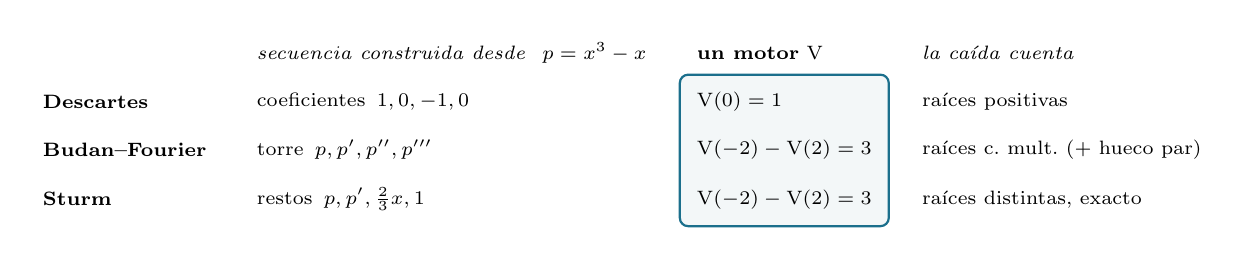
\begin{tikzpicture}[font=\scriptsize]
\matrix (m) [matrix of nodes, row sep=2.2mm, column sep=5mm, nodes={anchor=west, inner sep=2pt}]{
   & \textit{secuencia construida desde } $p=x^3-x$ & \textbf{un motor} $\V$ & \textit{la ca\'ida cuenta} \\
  \textbf{Descartes} & coeficientes $\,1,0,-1,0$ & $\V(0)=1$ & ra\'ices positivas \\
  \textbf{Budan--Fourier} & torre $\,p,p',p'',p'''$ & $\V(-2)-\V(2)=3$ & ra\'ices c.\ mult.\ ($+$ hueco par) \\
  \textbf{Sturm} & restos $\,p,p',\tfrac23 x,1$ & $\V(-2)-\V(2)=3$ & ra\'ices distintas, exacto \\
};
\begin{scope}[on background layer]
  \node[draw=ggteal,thick,rounded corners=3pt,fill=ggband!35,fit=(m-2-3)(m-4-3),inner sep=4pt] {};
\end{scope}
\end{tikzpicture}
\caption{Un polinomio, tres secuencias, un motor. Cada recuento cl\'asico es el \emph{mismo} motor de
variaci\'on de signos $\V$ aplicado a una secuencia distinta construida desde $p=x^3-x$: los coeficientes de
Descartes, la torre de derivadas de Budan--Fourier, los restos firmados de Sturm. Leen facetas
distintas---ra\'ices positivas, ra\'ices con multiplicidad, ra\'ices distintas---pero el recuento, su
constancia local fuera de los puntos cr\'iticos, y su telescopaje sobre $(a,b]$ son uno y el mismo (en
recuadro). Las escaleras detalladas est\'an en los papers compa\~neros~\cite{sturmlean,budanlean}; el sujeto
de este paper es la columna en recuadro que comparten.}
\label{fig:compare}
\end{figure}

\section{La l\'inea divisoria}\label{sec:divide}

Lo que separa a Sturm de Budan--Fourier no es cuesti\'on de gusto; es un axioma preciso, y la m\'aquina lo
hizo preciso. La \emph{cadena de Sturm} abstracta de Eisermann~\cite{eisermann} debe satisfacer una
condici\'on (su Def.~3.10): siempre que un miembro \emph{interior} $S_k$ se anula, sus vecinos son
estrictamente opuestos ah\'i,
\keyeq{S_k(c)=0\ \Longrightarrow\ S_{k-1}(c)\,S_{k+1}(c)<0\qquad(0<k<n),}
lo que en particular proh\'ibe que dos miembros consecutivos se anulen juntos. La cadena de Sturm lo
satisface (coprimalidad); la lectura de coeficientes de Descartes es degenerada pero compatible.

\begin{proposition}[la torre de derivadas no es una cadena de Sturm]\label{prop:notsturm}
La torre de derivadas falla el axioma de Eisermann en cada ra\'iz m\'ultiple. Concretamente, para
$p_A=(x-1)^2(x+1)$ con torre $\big[p_A,\,p_A',\,p_A'',\,p_A'''\big]$, el miembro interior $p_A'$ se anula en
$x=1$, pero
\[
  p_A(1)\cdot p_A''(1)=0\cdot4=0\ \not<\ 0,
\]
porque $p_A$ y $p_A'$ se anulan ah\'i \emph{a la vez}. Por tanto la torre no es una cadena de Sturm en el
sentido de~\cite{eisermann}, y la eliminaci\'on interior antipodal que prueba el teorema de Sturm no puede
aplicarse.
\end{proposition}

Este es todo el sentido de la ley por bloques. Donde una cadena de Sturm borra un miembro interior
ensanduichado cada vez (\lean{FlankReduce}), la torre debe resolver un bloque entero que se anula de una vez
(\lean{Rseq}/\lean{Lseq}: copia el signo de la derivada a la derecha, ni\'egalo a la izquierda). No son
t\'ecnicas rivales; la eliminaci\'on antipodal de uno en uno es el \emph{caso especial no degenerado} de la
ley por bloques, el caso en que cada bloque tiene longitud uno. La Figura~\ref{fig:divide} pone las dos
geometr\'ias locales lado a lado.

\begin{figure}[htbp]
\centering
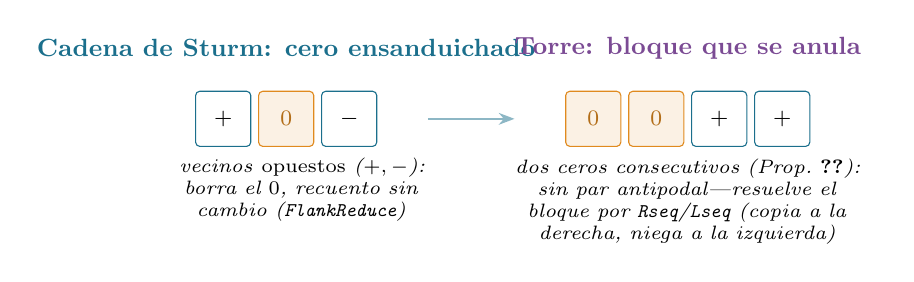
\begin{tikzpicture}[
  cell/.style={draw,rounded corners=1.5pt,minimum size=7mm,inner sep=1pt,font=\footnotesize},
  arr/.style={-{Stealth[length=2mm]},thick},
  lbl/.style={font=\scriptsize\itshape,align=center}]
  % Sturm side
  \node[font=\bfseries\small,text=ggteal] at (0.8,2.3) {Cadena de Sturm: cero ensanduichado};
  \node[cell,draw=ggteal] at (0,1.4) {$+$};
  \node[cell,draw=ggamber,fill=ggamber!12,text=ggamber!80!black] at (0.8,1.4) {$0$};
  \node[cell,draw=ggteal] at (1.6,1.4) {$-$};
  \node[lbl,text width=4.4cm] at (1.0,0.5)
    {vecinos \emph{opuestos} ($+,-$): borra el $0$, recuento sin cambio (\lean{FlankReduce})};
  % BF side
  \node[font=\bfseries\small,text=ggplum] at (5.9,2.3) {Torre: bloque que se anula};
  \node[cell,draw=ggamber,fill=ggamber!12,text=ggamber!80!black] at (4.7,1.4) {$0$};
  \node[cell,draw=ggamber,fill=ggamber!12,text=ggamber!80!black] at (5.5,1.4) {$0$};
  \node[cell,draw=ggteal] at (6.3,1.4) {$+$};
  \node[cell,draw=ggteal] at (7.1,1.4) {$+$};
  \node[lbl,text width=4.8cm] at (5.9,0.35)
    {dos ceros consecutivos (Prop.~\ref{prop:notsturm}): sin par antipodal---resuelve el bloque por
     \lean{Rseq}/\lean{Lseq} (copia a la derecha, niega a la izquierda)};
  \draw[arr,ggteal!50] (2.6,1.4) -- (3.7,1.4);
\end{tikzpicture}
\caption{Dos geometr\'ias locales. Izquierda: el cero interior de una cadena de Sturm est\'a entre signos
opuestos y se borra sin dejar rastro. Derecha: los ceros consecutivos de la torre no tienen tal s\'andwich;
el bloque se resuelve por colapso (derecha) y alternancia (izquierda). El primero es el caso especial de
longitud uno del segundo.}
\label{fig:divide}
\end{figure}

\section{Qu\'e es cl\'asico y qu\'e se aporta}\label{sec:ours}

Sin adornos. \emph{Cl\'asico, no nuestro}: que Descartes, Budan--Fourier y Sturm son facetas de un mismo
principio de variaci\'on de signos (Akritas~\cite{akritas}; Basu--Pollack--Roy~\cite{bpr}); el \'indice de
Cauchy como el invariante unificador profundo (Cauchy; Eisermann~\cite{eisermann}); y la axiomatizaci\'on
abstracta de cadenas de Sturm en s\'i~\cite{eisermann}. \emph{Ya verificado por m\'aquina en otro sitio}: la
v\'ia del \'indice de Cauchy, en Isabelle/HOL, por Li y Paulson~\cite{liCauchy}; y el teorema de
Budan--Fourier, en Isabelle/HOL, por Li~\cite{liBF}. \emph{Aportado aqu\'i}: el motor compartido de
variaci\'on de signos, expl\'icito, en Lean~4 sobre Mathlib; las primeras formalizaciones en Lean del teorema
de Sturm~\cite{sturmlean} y de Budan--Fourier~\cite{budanlean} que pasan por \'el; el puente
\lean{fourierVar p 0 = Polynomial.signVariations p} (\lean{Descartes.lean}), que identifica el $\V(0)$ del
motor con el recuento de signos de coeficientes sobre el que est\'a enunciada la propia regla de Descartes de
Mathlib---de modo que el tercer recuento se verifica contra la biblioteca, no se lee solo en prosa; y la
Proposici\'on~\ref{prop:notsturm}, la colocaci\'on precisa de la torre de derivadas \emph{fuera} del axioma
cl\'asico de cadena de Sturm, con \lean{Rseq}/\lean{Lseq} identificadas como la ley local de ese r\'egimen
m\'as amplio. Todo es sobre $\R$; el paso de multiplicidad usa caracter\'istica cero de forma esencial. Nunca
se calcula una ra\'iz; no se produce certificado; no se construye aislador.

\section{Preguntas que merece la pena llevarse}\label{sec:open}

\begin{enumerate}\itemsep3pt
\item \emph{El axioma m\'as d\'ebil.} La Proposici\'on~\ref{prop:notsturm} muestra que la torre escapa de
la condici\'on de Eisermann. ¿Cu\'al es la hip\'otesis \emph{m\'as d\'ebil} sobre una secuencia abstracta bajo
la que sigue valiendo la ley local $\V(c^-)=\V(c^+)+\mu_c+2e$---una que tenga el axioma antipodal de cadena de
Sturm y la torre de derivadas como sus dos instancias principales? Una estructura Lean que cargue exactamente
esa hip\'otesis sostendr\'ia el lema local una vez en vez de tres. El motor de la Secci\'on~\ref{sec:engine}
es ya esa estructura menos la ley local; la ley es lo que pide axiomatizarse.
\item \emph{A trav\'es del \'indice de Cauchy.} Li y Paulson formalizaron el \'indice de Cauchy en
Isabelle~\cite{liCauchy}; Mathlib no tiene tal desarrollo. ¿Factoriza el motor de aqu\'i a trav\'es de un
\'indice de Cauchy en Lean, recuperando Sturm y Budan--Fourier como c\'alculos de n\'umero de vueltas en el
sentido de~\cite{eisermann}---y aparecer\'ia entonces la torre de derivadas como un caso frontera no gen\'erico
tambi\'en all\'i?
\item \emph{De cota a certificado.} El excedente par mide cu\'anto se pasa Budan--Fourier. ¿Puede bisecar
hasta que se anule convertirse en un aislador de ra\'ices verificado y productor de certificados sobre Mathlib,
el an\'alogo consciente de la multiplicidad de los m\'etodos de Vincent--Collins--Akritas~\cite{collinsakritas}?
\end{enumerate}

\noindent El patr\'on que recorre los tres es una reflexi\'on: el teorema es ahora un punto fijo que un
n\'ucleo defiende, as\'i que la direcci\'on viva no es reprobarlo sino hallar la \emph{\'unica} hip\'otesis de
la que los tres recuentos---y quiz\'a el \'indice de Cauchy por encima de ellos---son instancias, y aprender
exactamente cu\'anto la fuerzan a debilitarse los bloques de la torre de derivadas.

\section*{Reproducir}
\begin{verbatim}
git clone https://github.com/karlesmarin/godsil-gutman-lean
cd godsil-gutman-lean && lake exe cache get
lake env lean Sturm.lean          # el motor compartido + instancia de Sturm
lake env lean BudanFourier.lean   # la instancia de Budan-Fourier (importa Sturm)
lake env lean Descartes.lean      # el puente de Descartes: V(0) = signVariations
\end{verbatim}
Lean \lean{v4.30.0-rc2}, pin de Mathlib \lean{701fb6e9}. Todos los teoremas cabecera son \lean{sorry}-free y
\lean{\#print axioms} reporta solo \lean{propext}, \lean{Classical.choice}, \lean{Quot.sound}. Los signos
trabajados de cada figura se re-derivan en aritm\'etica exacta antes de dibujar la figura (\lean{figures/}).

\begin{thebibliography}{99}\small
\bibitem{descartes} R.~Descartes, \emph{La G\'eom\'etrie} (1637).
\bibitem{budan} F.~D.~Budan de Boislaurent, \emph{Nouvelle m\'ethode pour la r\'esolution des
\'equations num\'eriques}, Par\'is (1807).
\bibitem{fourier} J.~Fourier, \emph{Analyse des \'equations d\'etermin\'ees}, Firmin Didot, Par\'is
(p\'ostumo, 1831).
\bibitem{sturm} C.~Sturm, M\'emoire sur la r\'esolution des \'equations num\'eriques, \emph{M\'em.\
pr\'esent\'es par divers savants \`a l'Acad.\ Royale des Sci.} \textbf{6} (1835) 271--318.
\bibitem{akritas} A.~G.~Akritas, Reflections on a pair of theorems by Budan and Fourier, \emph{Math.\
Magazine} \textbf{55} (1982) 292--298.
\bibitem{collinsakritas} G.~E.~Collins, A.~G.~Akritas, Polynomial real root isolation using Descartes'
rule of signs, en \emph{Proc.\ SYMSAC~'76}, ACM, 1976, 272--275.
\bibitem{bpr} S.~Basu, R.~Pollack, M.-F.~Roy, \emph{Algorithms in Real Algebraic Geometry}, 2.\textsuperscript{a}
ed., Springer, 2006 (teor\'ia de variaci\'on de signos, Cap.~2).
\bibitem{eisermann} M.~Eisermann, The fundamental theorem of algebra made effective: an elementary
real-algebraic proof via Sturm chains, \emph{Amer.\ Math.\ Monthly} \textbf{119} (2012), no.~9,
715--752; \texttt{arXiv:0808.0097}.
\bibitem{liBF} W.~Li, L.~C.~Paulson, Counting polynomial roots in Isabelle/HOL: a formal proof of the
Budan--Fourier theorem, en \emph{CPP~2019}, ACM, 2019, 52--64; \texttt{arXiv:1811.11093}.
\bibitem{liCauchy} W.~Li, L.~C.~Paulson, Evaluating winding numbers and counting complex roots through
Cauchy indices in Isabelle/HOL, \emph{J.~Automated Reasoning} \textbf{64} (2020), no.~2, 331--360;
\texttt{arXiv:1804.03922}.
\bibitem{mathlib} The mathlib Community, The Lean mathematical library, en \emph{CPP~2020}, ACM, 2020,
367--381.
\bibitem{lean4} L.~de Moura, S.~Ullrich, The Lean~4 theorem prover and programming language, en
\emph{CADE~28}, LNCS \textbf{12699}, Springer, 2021, 625--635.
\bibitem{sturmlean} C.~Mar\'in, \emph{The Staircase of Signs: Sturm's Root-Counting Theorem,
Machine-Checked in Lean~4}, Zenodo, 2026, \texttt{doi:10.5281/zenodo.20707348}.
\bibitem{budanlean} C.~Mar\'in, \emph{Counting with the Derivative Tower: The Budan--Fourier Theorem,
Machine-Checked in Lean~4}, 2026 (paper compa\~nero).
\end{thebibliography}

\end{document}
